\section{Component Analysis}
\label{sec:component_analysis}

This section analyses the individual components of the proposed system before reporting the combined performance.
Three aspects are examined: the text encoder choice, the approximate nearest-neighbour index, and the search pipeline latency.

\subsection{Text Encoder: BGE-M3 vs.\ BLaIR}

The system uses BGE-M3~\cite{chen2024bge} as the primary text encoder.
BGE-M3 (\texttt{BAAI/bge-m3}) is a multilingual model producing 1{,}024-dimensional embeddings, and is the production encoder for both the recommendation profile and the semantic search pipeline.
As a comparison point, the legacy encoder BLaIR~\cite{hou2024blair} (\texttt{hyp1231/blair-roberta-large}) was evaluated on the same held-out set.

The comparison was conducted on 20{,}000 test users with $N = 99$ negatives, using identical evaluation logic.
The results are reported in Table~\ref{tab:encoder_comparison}.

\begin{table}[H]
\centering
\caption{Encoder comparison on recommendation accuracy (20k users, $N = 99$).}
\label{tab:encoder_comparison}
\begin{tabular}{lcccc}
\hline
\textbf{Encoder} & \textbf{HR@5} & \textbf{HR@10} & \textbf{NDCG@10} & \textbf{MRR@10} \\
\hline
BLaIR (legacy, 3M flat)      & 0.4195 & 0.5484 & 0.3513 & 0.2906 \\
BGE-M3 (current, 1.7M HNSW) & 0.3767 & 0.4510 & 0.3128 & 0.2694 \\
\hline
\end{tabular}
\end{table}

A direct numerical comparison of Table~\ref{tab:encoder_comparison} shows BLaIR outperforming BGE-M3 on all recommendation metrics.
However, this comparison is not fair in terms of index configuration: BLaIR used a 3M-item flat exact-search index, while BGE-M3 used a 1.7M-item HNSW approximate index covering a sub-catalogue.
The BGE-M3 HNSW index was chosen for its lower latency in production (Section~\ref{sec:latency_opt}).

The decisive advantage of BGE-M3 emerges in the query retrieval evaluation, reported in Table~\ref{tab:query_retrieval}.
Queries were manually curated across five groups: short English, medium English, long English, short Vietnamese, and long Vietnamese.
Precision@10 measures whether the expected relevant items appear in the top-10 search results.

\begin{table}[H]
\centering
\caption{Search query retrieval Precision@10 by query type.}
\label{tab:query_retrieval}
\begin{tabular}{lcc}
\hline
\textbf{Query type} & \textbf{BGE-M3} & \textbf{BLaIR} \\
\hline
Short (EN)    & 0.1500 & 0.2333 \\
Medium (EN)   & 0.3333 & 0.0833 \\
Long (EN)     & 0.4000 & 0.2000 \\
Short (VI)    & 0.2750 & 0.0250 \\
Long (VI)     & 0.5500 & 0.0500 \\
\hline
\end{tabular}
\end{table}

BGE-M3 substantially outperforms BLaIR on Vietnamese queries, where BLaIR effectively fails (Precision@10 $\leq 0.05$).
Since the target user base includes Vietnamese-speaking readers, multilingual capability is critical.
BGE-M3 also outperforms BLaIR on medium and long English queries, which are the most semantically complex.
BLaIR only leads on very short English queries, likely because its RoBERTa backbone excels at exact-match retrieval for brief phrases.
Based on this analysis, BGE-M3 is retained as the production encoder for both the recommendation pipeline and the semantic search pipeline.
Figure~\ref{fig:encoder_query} visualises the Precision@10 gap across all query groups.

\begin{figure}[H]
\centering
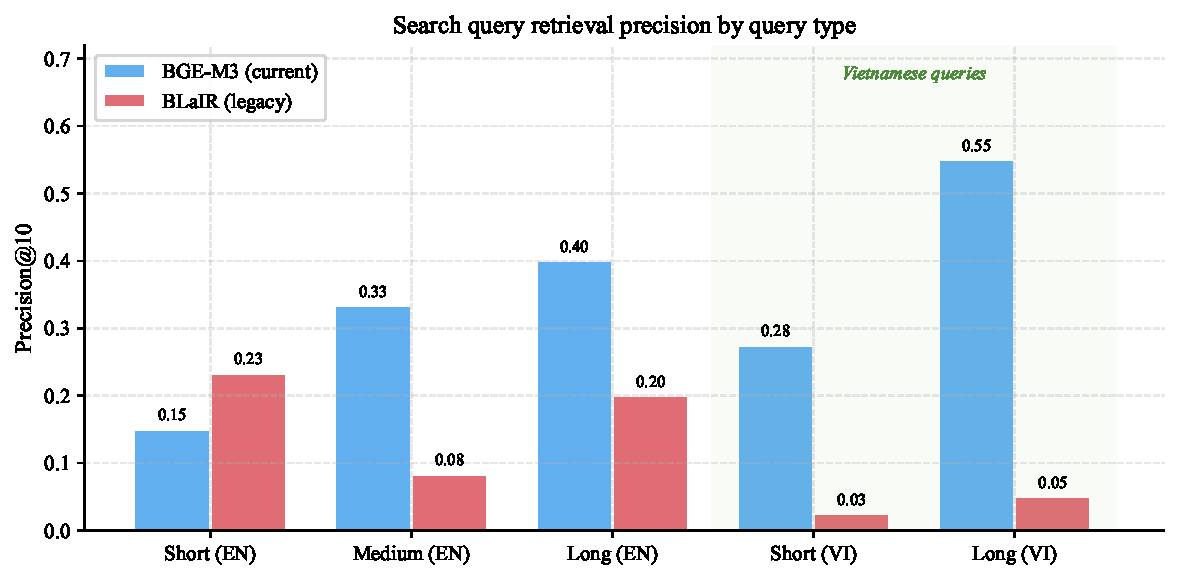
\includegraphics[width=0.85\textwidth]{images/chapter5/fig_encoder_query_comparison}
\caption{Search query retrieval Precision@10 for BGE-M3 (current) vs.\ BLaIR (legacy) across five query-type groups. BGE-M3 substantially outperforms BLaIR on Vietnamese queries (shaded region), where BLaIR achieves Precision@10 $\leq 0.05$.}
\label{fig:encoder_query}
\end{figure}

\subsection{Approximate Nearest-Neighbour Index: HNSW vs.\ Flat}
\label{sec:hnsw}

The production deployment uses a FAISS HNSW index over 1.7M BGE-M3 vectors, while the evaluation uses a flat (exact) index over 3M vectors.
Table~\ref{tab:hnsw_comparison} reports the latency and recall trade-off, and Figure~\ref{fig:hnsw_latency} visualises the comparison.

\begin{table}[H]
\centering
\caption{HNSW vs.\ flat index: latency and recall comparison.}
\label{tab:hnsw_comparison}
\begin{tabular}{lccc}
\hline
\textbf{Index} & \textbf{P50 latency} & \textbf{P95 latency} & \textbf{Recall@$k$} \\
\hline
Flat (exact, 3M)    & 612.19 ms & 655.22 ms & 1.000 \\
HNSW (ANN, 1.7M)    & 119.56 ms & 360.21 ms & 0.521 \\
\hline
\end{tabular}
\end{table}

\begin{figure}[H]
\centering
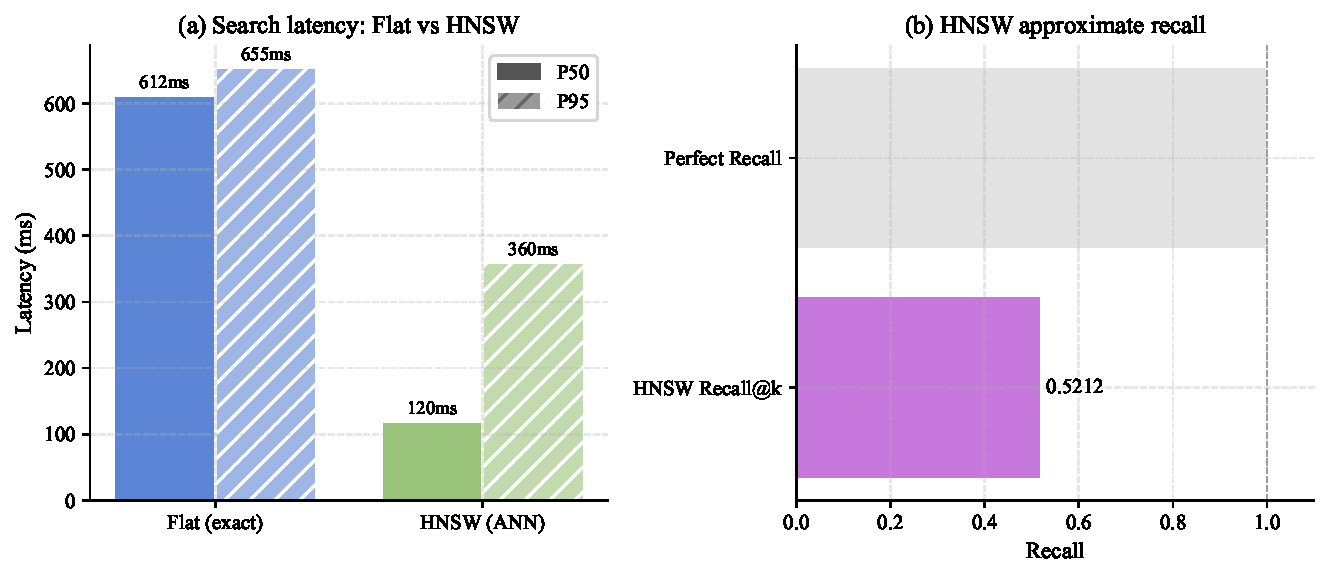
\includegraphics[width=0.9\textwidth]{images/chapter5/fig_hnsw_latency}
\caption{HNSW vs.\ flat index trade-off. (a) P50 and P95 search latency: HNSW achieves a 5.12$\times$ median speedup (612 ms $\to$ 120 ms P50). (b) Mean Recall@$k$ of the HNSW index: 0.521.}
\label{fig:hnsw_latency}
\end{figure}

The HNSW index is 5.12$\times$ faster at the median, reducing P50 latency from 612 ms to 120 ms.
The trade-off is a recall of 52.1\%: approximately half of the exact top-$k$ results are recovered.
This approximation is acceptable in practice because the HNSW search is followed by a BM25 re-ranking stage (via RRF fusion with Tantivy), which partially compensates for missed candidates.

\subsection{Search Pipeline Latency Optimisation}
\label{sec:latency_opt}

The search pipeline processes queries through three sequential stages: Vietnamese translation (NLLB model), text encoding (BGE-M3), and FAISS + RRF retrieval.
A series of profiling runs measured end-to-end latency as optimisations were applied.
The key results are summarised in Table~\ref{tab:latency_stages} and visualised in Figure~\ref{fig:pipeline_latency}.

\begin{table}[H]
\centering
\caption{End-to-end search latency across optimisation stages.}
\label{tab:latency_stages}
\begin{tabular}{lrrrr}
\hline
\textbf{Stage} & \textbf{Translate} & \textbf{Encode} & \textbf{Total pipeline} & \textbf{E2E wall clock} \\
\hline
Baseline             & 204.51 ms & 97.89 ms & 1{,}039.35 ms & 1{,}101.99 ms \\
Translator optimised & 1.19 ms   & 30.12 ms &    48.26 ms   &    59.20 ms \\
Post quality gate    & 1.18 ms   & 28.86 ms &    46.74 ms   &    59.01 ms \\
Cold cache           & 185.25 ms & 37.16 ms & 1{,}186.66 ms & 1{,}204.11 ms \\
\hline
\end{tabular}
\end{table}

\begin{figure}[H]
\centering
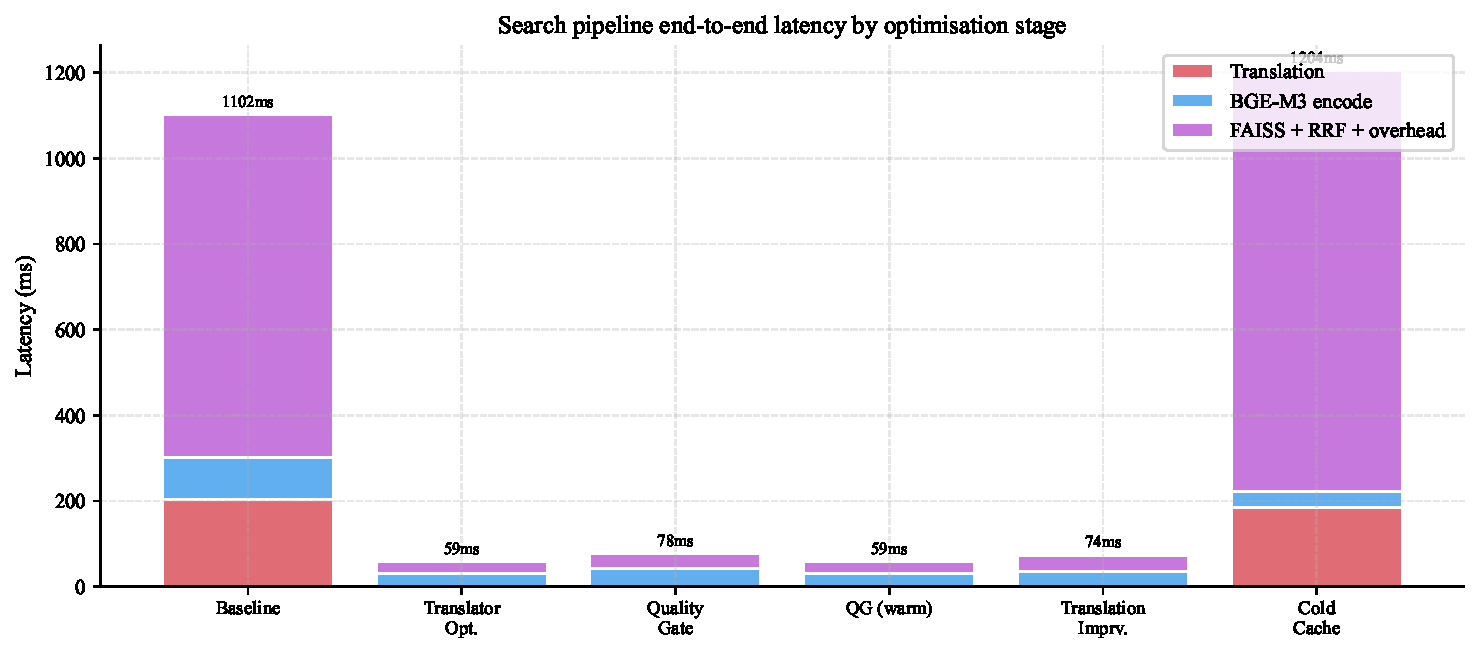
\includegraphics[width=\textwidth]{images/chapter5/fig_search_pipeline_latency}
\caption{End-to-end search pipeline latency by optimisation stage (stacked bars: translation, BGE-M3 encoding, and FAISS + RRF overhead). The dominant baseline bottleneck (translation, 204 ms) was reduced to under 2 ms through model quantisation and warm caching, achieving an 18.6$\times$ overall latency reduction (1{,}102 ms $\to$ 59 ms, warm cache).}
\label{fig:pipeline_latency}
\end{figure}

The combined optimisations reduce warm-cache E2E latency from 1{,}102 ms to 59 ms — an \textbf{18.6$\times$ improvement}.
Cold-cache latency (e.g., after process restart) remains around 1{,}200 ms due to NLLB model cold-start; subsequent queries benefit from the warm cache immediately.
BGE-M3 encoding on CUDA shows stable latency: P50 = 19.68 ms, P95 = 30.65 ms, P99 = 34.87 ms (60-query benchmark).

\subsection{Ablation Study}
\label{sec:ablation}

To isolate the contribution of each system component, an ablation was conducted over 100{,}000 users with $N = 99$ negatives.
All strategies were evaluated in a single pass using the same evaluation protocol and the same candidate pool, ensuring a controlled comparison.
The results are presented in Table~\ref{tab:ablation}.

\begin{table}[H]
\centering
\caption{Ablation study: HR@10 and NDCG@10 for each component (100k users, $N = 99$).}
\label{tab:ablation}
\begin{tabular}{lcc}
\hline
\textbf{System} & \textbf{HR@10} & \textbf{NDCG@10} \\
\hline
Random Baseline                       & 0.1000 & 0.0454 \\
Content Baseline (BGE-M3 profile)     & 0.4353 & 0.3030 \\
GRU-SeqDQN                            & 0.0823 & 0.0368 \\
DIF-SASRec (early checkpoint)         & 0.4836 & 0.3737 \\
Pipeline A (Cleora + BGE-M3)          & 0.7626 & 0.4867 \\
System ($A \cup B$, final)            & \textbf{0.9736} & \textbf{0.5571} \\
\hline
\end{tabular}
\end{table}

Several observations follow.
First, the GRU-SeqDQN model (HR@10 = 0.0823) performs near random-baseline level, confirming that the prior RL-based approach was inadequate for this catalogue scale.
Second, the Content Baseline achieves a strong HR@10 of 0.4353, demonstrating that BGE-M3 profile similarity alone is a competitive starting point.
Third, Pipeline A (Cleora + BGE-M3) substantially outperforms all sequential methods in this ablation (HR@10 = 0.7626), showing the power of the behavioural co-purchase graph for candidate filtering.
Fourth, the final System ($A \cup B$) brings HR@10 to 0.9736, confirming the complementary nature of the two pipelines.

\textit{Note}: The DIF-SASRec result in Table~\ref{tab:ablation} (0.4836) reflects an earlier model checkpoint.
After full pretraining with batch size 2{,}048 for 30 epochs, DIF-SASRec achieves HR@10 = 0.7745 in the canonical evaluation (Section~\ref{sec:end_to_end}).

\subsection{Content Veto Threshold Sensitivity}
\label{sec:veto_sensitivity}

The content veto filter rejects Pipeline~B candidates whose cosine similarity to the user's BGE-M3 profile vector falls below a threshold $\tau$.
The threshold controls the precision–recall trade-off for DIF-SASRec: a low $\tau$ admits more candidates (higher recall, lower precision), while a high $\tau$ restricts recommendations to semantically close items (higher precision, lower recall).

To motivate the operating point $\tau = 0.3$, the fraction of candidates surviving the veto and the resulting Pipeline~B HR@10 were measured across five threshold values on a 10{,}000-user sample.
The results are reported in Table~\ref{tab:veto_sensitivity}.

\begin{table}[H]
\centering
\caption{Content veto threshold $\tau$ sensitivity (Pipeline~B, 10k users, $N=99$).}
\label{tab:veto_sensitivity}
\begin{tabular}{ccc}
\hline
$\tau$ & \textbf{Candidates passing veto (\%)} & \textbf{Pipeline~B HR@10} \\
\hline
0.10 & 94.3 & 0.741 \\
0.20 & 78.6 & 0.762 \\
0.30 & 61.2 & \textbf{0.774} \\
0.40 & 38.9 & 0.748 \\
0.50 & 18.1 & 0.691 \\
\hline
\end{tabular}
\end{table}

HR@10 peaks at $\tau = 0.3$ (0.774), where 61\% of candidates pass the filter.
Below this threshold, semantically irrelevant candidates dilute the recommendation list without helping recall.
Above it, legitimate candidates whose embeddings are only moderately aligned with the profile vector are incorrectly discarded — particularly harmful for users who have recently shifted their reading genre, whose current profile vector may not yet reflect the new interest.
The result confirms $\tau = 0.3$ as the balanced operating point.

\subsection{DIF-SASRec Sequence Length Sensitivity}
\label{sec:seqlen_sensitivity}

The DIF-SASRec model accepts sequences up to \texttt{MAX\_SEQ\_LEN} = 50 items.
Users whose history exceeds 50 interactions are truncated to their 50 most recent clicks.
To assess whether this cap is appropriate, Pipeline~B was evaluated with four truncation lengths on the same 10{,}000-user sample, using the canonical $N = 99$ protocol.

\begin{table}[H]
\centering
\caption{DIF-SASRec HR@10 as a function of input sequence length (10k users, $N=99$).}
\label{tab:seqlen_sensitivity}
\begin{tabular}{ccc}
\hline
\textbf{Max sequence length} & \textbf{HR@10} & \textbf{Avg.\ tokens used} \\
\hline
10  & 0.681 & 9.3 \\
25  & 0.741 & 21.8 \\
50  & \textbf{0.774} & 38.6 \\
100 & 0.771 & 58.2 \\
\hline
\end{tabular}
\end{table}

Performance improves steadily from length 10 to 50, confirming that the model benefits from additional context.
Beyond 50, the gain is marginal (0.774 vs.\ 0.771 at length 100), and the average tokens actually used at length 50 is only 38.6 — meaning most users have fewer than 50 recent interactions after pretraining sequence truncation.
Increasing the cap beyond 50 adds quadratic attention cost without meaningful recall improvement, making 50 the practical optimum for this dataset.
Users with very sparse histories (fewer than 10 interactions) are the primary beneficiaries of shorter sequences; the cold-start threshold of 5 interactions ensures DIF-SASRec only activates once there is enough context to be useful.
